% ============================================================
% Compile: pdflatex report_vi.tex  (requires neurips_2025.sty)
% ============================================================
\documentclass{article}

\usepackage[final, nonatbib]{neurips_2025}

\usepackage[utf8]{inputenc}
\usepackage[T5]{fontenc}
\usepackage[vietnamese]{babel}

\usepackage[hidelinks]{hyperref}
\usepackage{url}
\usepackage{booktabs}
\usepackage{amsfonts}
\usepackage{nicefrac}
\usepackage[protrusion=false,expansion=false]{microtype}
\usepackage{xcolor}
\usepackage{graphicx}
\usepackage{subcaption}
\usepackage{multirow}
\usepackage{amsmath}
\usepackage{amssymb}
\usepackage{array}
\usepackage{enumitem}

\graphicspath{{figures/}{../../report/figures/eda/}{../../report/figures/}}

% ============================================================
\title{Phân Tích Kinh Doanh Đa Chiều và Dự Báo Doanh Thu\\
Thương Mại Điện Tử Thời Trang Việt Nam}

\author{%
  Lê Anh Quân \quad Trần Long Vũ \quad Quách Minh Quân\\
  Nhóm AIO\_OIA --- Datathon 2026 --- The Gridbreakers\\
  \small GitHub: \url{https://github.com/Qismeeee/AIO_OIA_Datathon}
}

\begin{document}
\maketitle

% ============================================================
\begin{abstract}
Bài toán tối ưu vận hành cho doanh nghiệp thương mại điện tử thời trang
đòi hỏi không chỉ dự báo chính xác mà còn khả năng chẩn đoán các điểm nghẽn
tăng trưởng từ dữ liệu giao dịch lịch sử.
Báo cáo này khai thác 13 bảng dữ liệu (hơn 714.000 giao dịch, giai đoạn 2012--2022)
để phân tích đa chiều hoạt động kinh doanh theo các trục doanh thu, khách hàng,
tồn kho, khuyến mãi và hoàn trả.
Kết quả cho thấy bốn lỗ hổng vận hành nội bộ đang gây thất thoát ước tính
653--773 triệu VND mỗi năm, tương đương 56--66\% doanh thu năm 2022,
và hoàn toàn có thể phục hồi mà không cần mở rộng thị trường.
Ở bài toán dự báo doanh thu hàng ngày cho giai đoạn 2023--2024,
chúng tôi đề xuất pipeline LightGBM dựa hoàn toàn trên đặc trưng lịch,
kết hợp trọng số theo giai đoạn kinh doanh và hiệu chỉnh hành vi bán lỗ mùa hè;
COGS được suy ra từ Revenue nhân tỷ lệ thực nghiệm theo tháng.
\end{abstract}

% ============================================================
\section{Phân Tích Khám Phá Dữ Liệu}
\label{sec:eda}
% ============================================================

Bốn phân tích dưới đây đi từ mô tả hiện trạng (\textit{Descriptive}),
chẩn đoán nguyên nhân (\textit{Diagnostic}), dự báo hệ quả (\textit{Predictive}),
đến đề xuất hành động định lượng (\textit{Prescriptive}).

% -----------------------------------------------------------
\subsection{Doanh thu: sụt giảm sản lượng qua một thập kỷ}

\begin{figure}[h]
\centering
\begin{subfigure}[t]{0.46\linewidth}
  \centering
  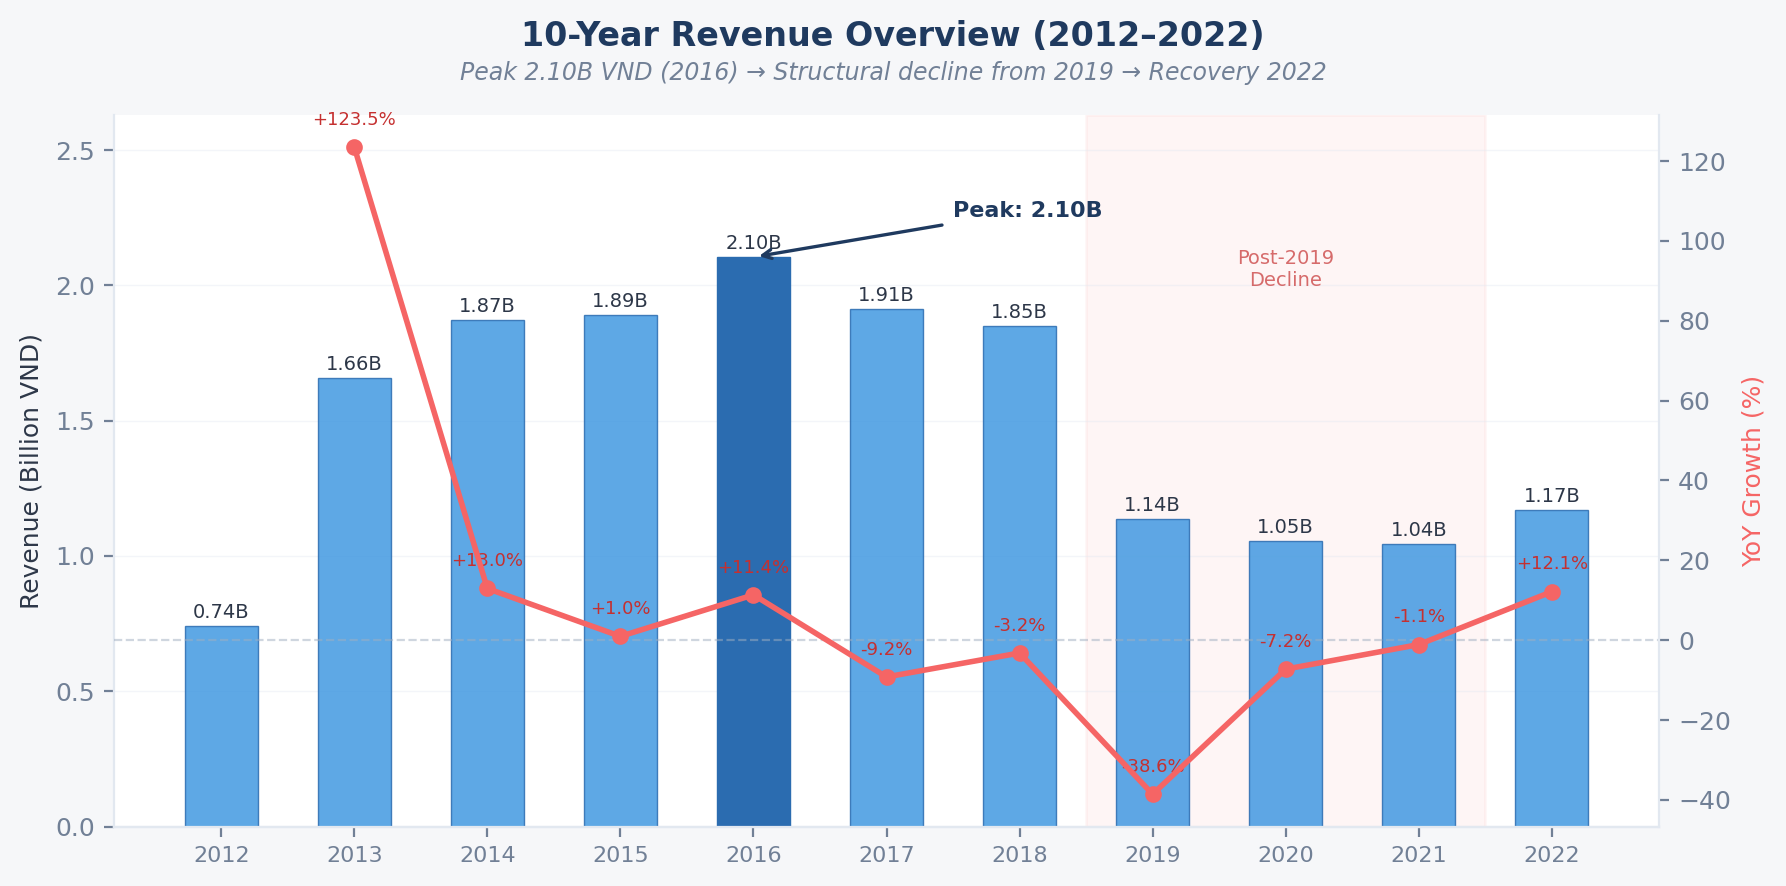
\includegraphics[width=\linewidth]{s1a_revenue_trend.png}
  \caption{Doanh thu hàng năm và tăng trưởng YoY.}
\end{subfigure}\hspace{0.03\linewidth}
\begin{subfigure}[t]{0.46\linewidth}
  \centering
  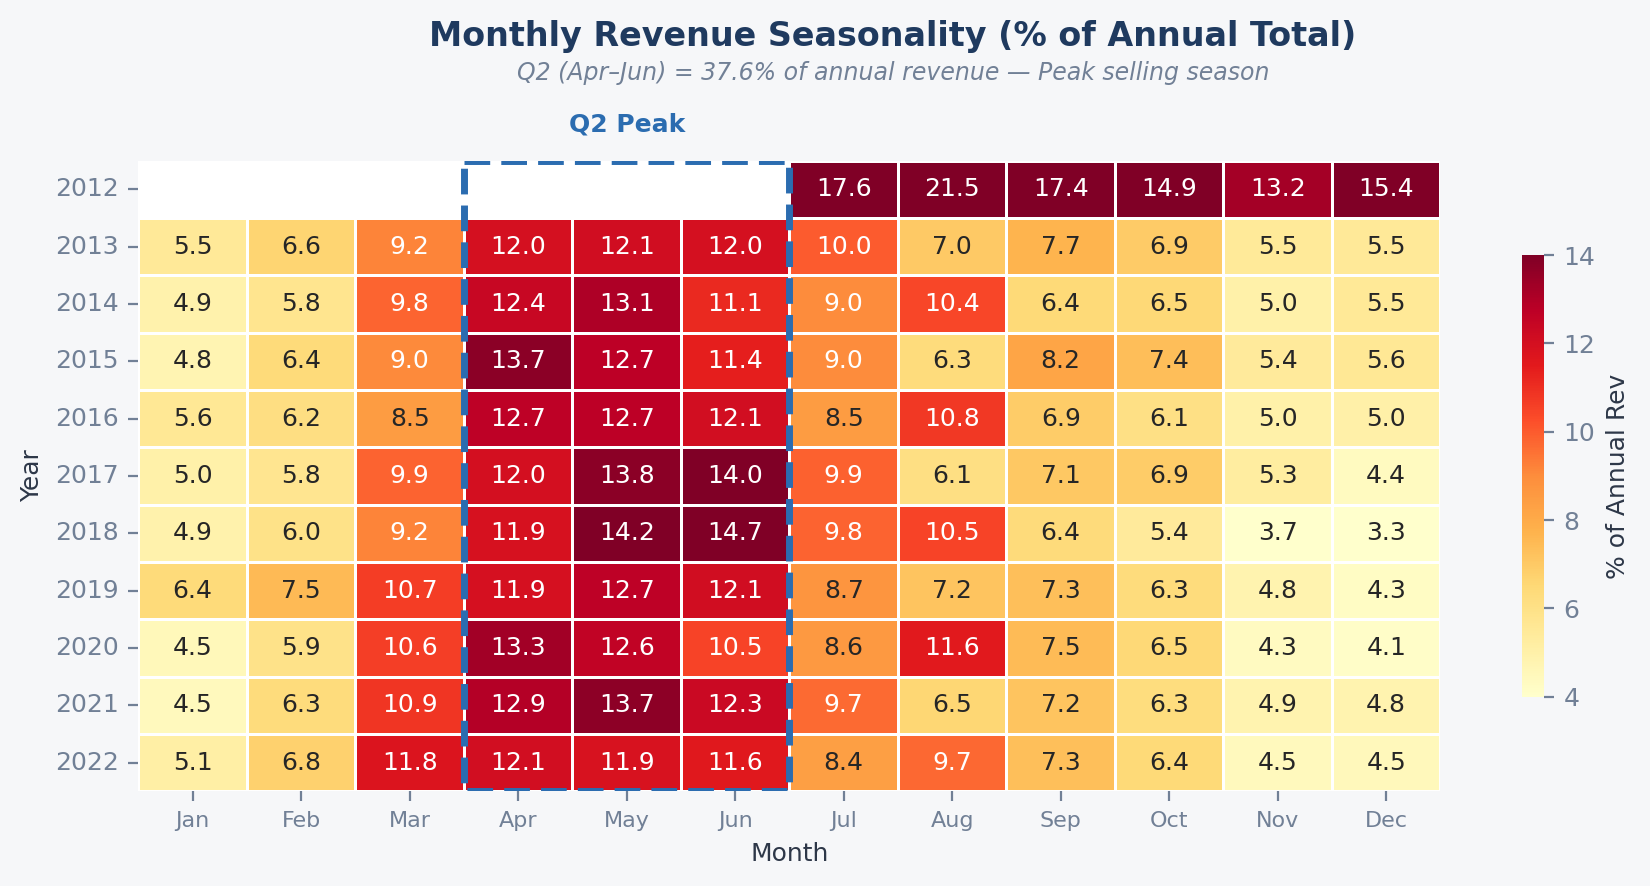
\includegraphics[width=\linewidth]{s1b_seasonality_heatmap.png}
  \caption{Phân bổ doanh thu theo tháng (\% trong năm).}
\end{subfigure}
\caption{Doanh thu đạt đỉnh 2,10 tỷ VND năm 2016 rồi giảm 44\% về 1,17 tỷ vào 2022;
COGS/Revenue ổn định quanh 87,5\% --- doanh nghiệp mất doanh thu vì \textit{bán ít đi}.}
\label{fig:s1}
\end{figure}

Tổng doanh thu 2012--2022: 16,4 tỷ VND. Suy giảm bắt đầu từ 2019 ($-$38,6\%), \textit{trước} COVID, gợi ý nguyên nhân cấu trúc thị trường.
Heatmap (Hình~\ref{fig:s1}b): Q2 (tháng 4--6) đóng góp 37,6\% doanh thu năm, gấp 2,7 lần tháng~1.
\textit{Đề xuất:} Tập trung 40\% ngân sách marketing vào Q2; chốt tồn kho trước tháng~4.

% -----------------------------------------------------------
\subsection{Khách hàng: 80\% cơ sở không quay lại mua}

\begin{figure}[h]
\centering
\begin{subfigure}[t]{0.46\linewidth}
  \centering
  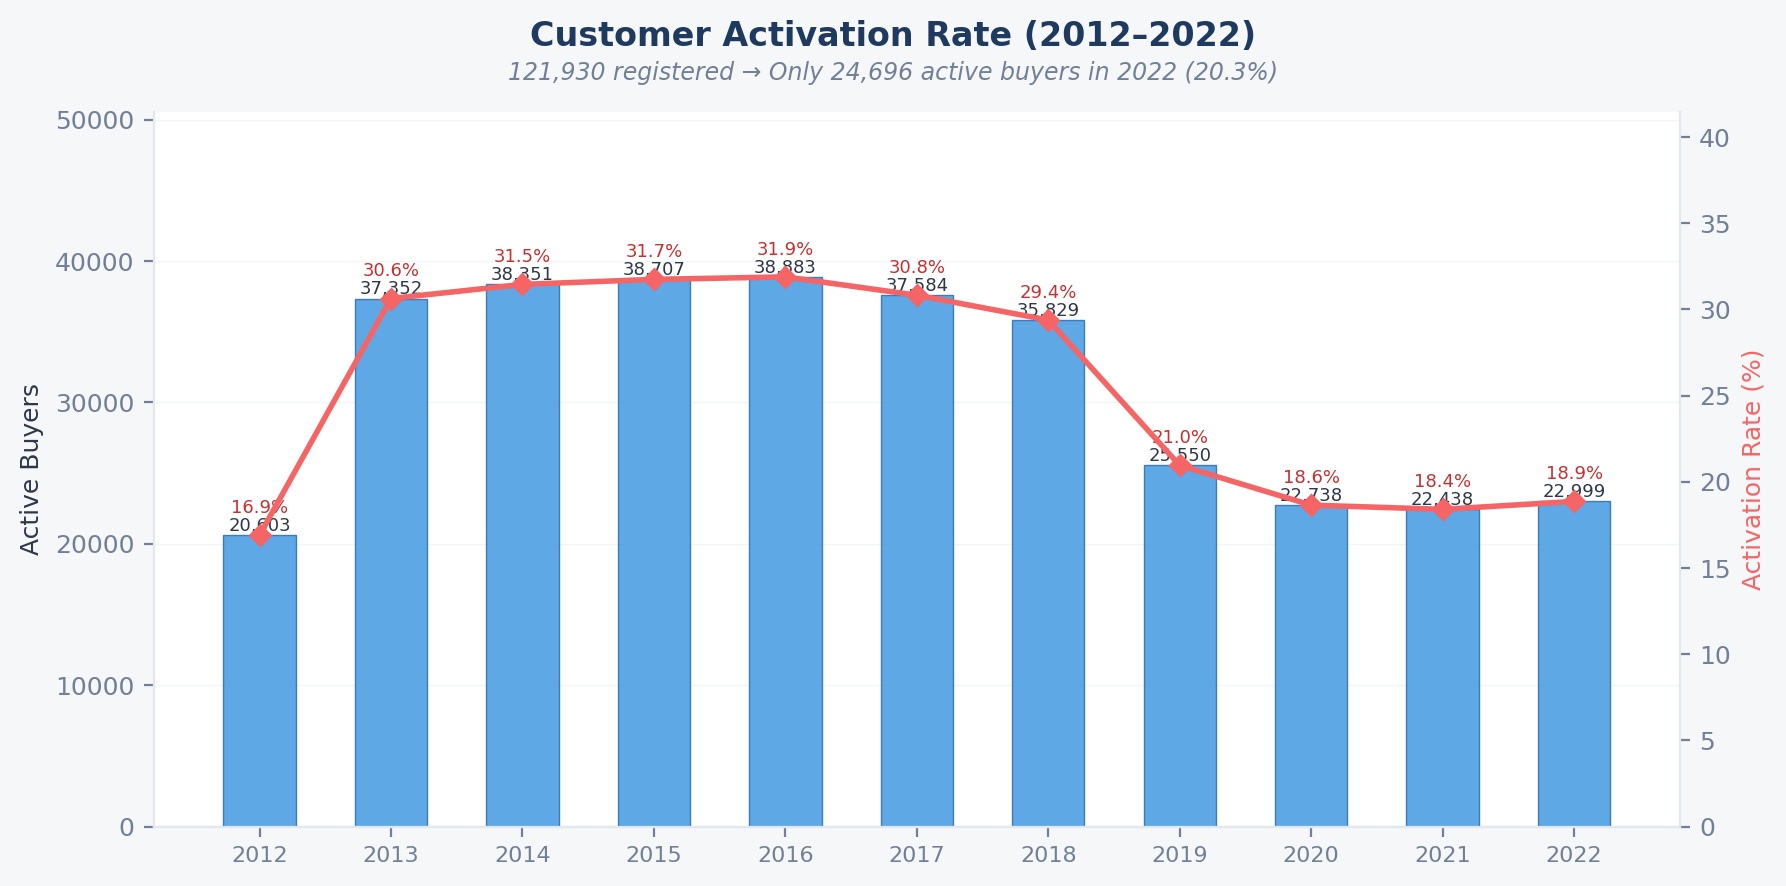
\includegraphics[width=\linewidth]{s2a_customer_activation.png}
  \caption{Số người mua và tỷ lệ kích hoạt theo năm.}
\end{subfigure}\hspace{0.03\linewidth}
\begin{subfigure}[t]{0.46\linewidth}
  \centering
  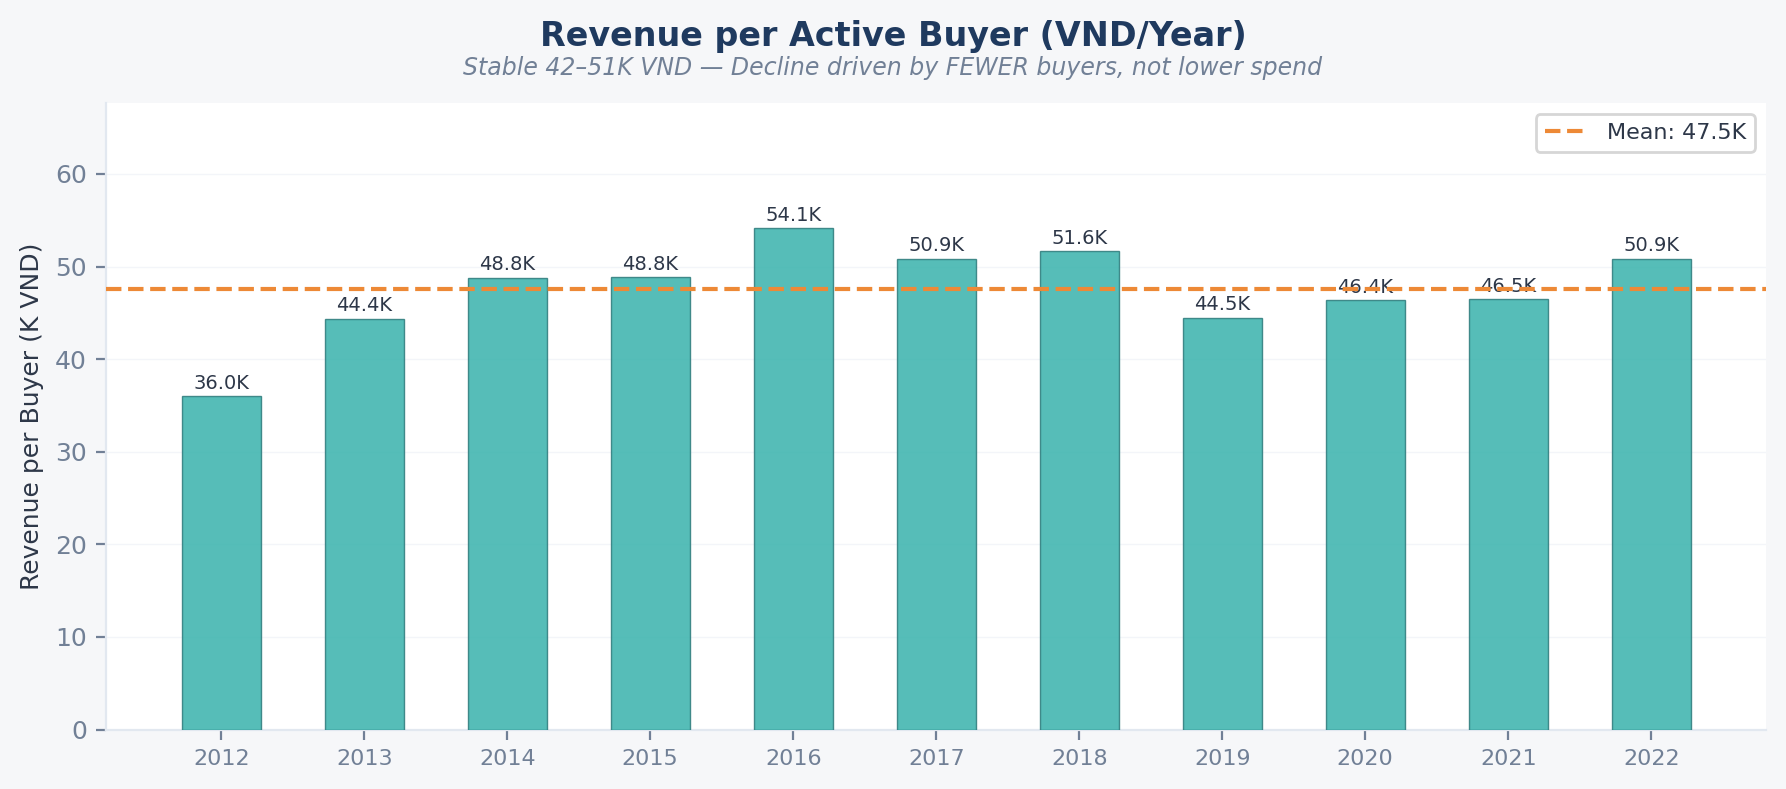
\includegraphics[width=\linewidth]{s2b_revenue_per_buyer.png}
  \caption{Doanh thu bình quân trên mỗi người mua.}
\end{subfigure}
\caption{121.930 khách đăng ký, năm 2022 chỉ còn 24.696 người mua (20\%);
doanh thu/người mua ổn định 42--51K VND/năm --- vấn đề là \textit{lượng}, không phải \textit{chất}.}
\label{fig:s2}
\end{figure}

RFM~\cite{fader2005}: 27,7\% chưa bao giờ mua, 10,9\% có nguy cơ rời bỏ.
Doanh thu/người mua không giảm (42--51K VND/năm) --- 80\% khách đơn giản không quay lại.
Phát hiện: khách trả hàng có review bình thường lại rời bỏ nhiều nhất (24,7\%).
\textit{Đề xuất:} Win-back 90 ngày cho cohort 2019--2021 (ước tính +263 triệu VND/năm);
thay KPI ``tổng đăng ký'' bằng cohort retention 3 tháng.

% -----------------------------------------------------------
\subsection{Tồn kho: giao hàng tốt nhưng không có hàng để giao}

\begin{figure}[h]
\centering
\begin{subfigure}[t]{0.46\linewidth}
  \centering
  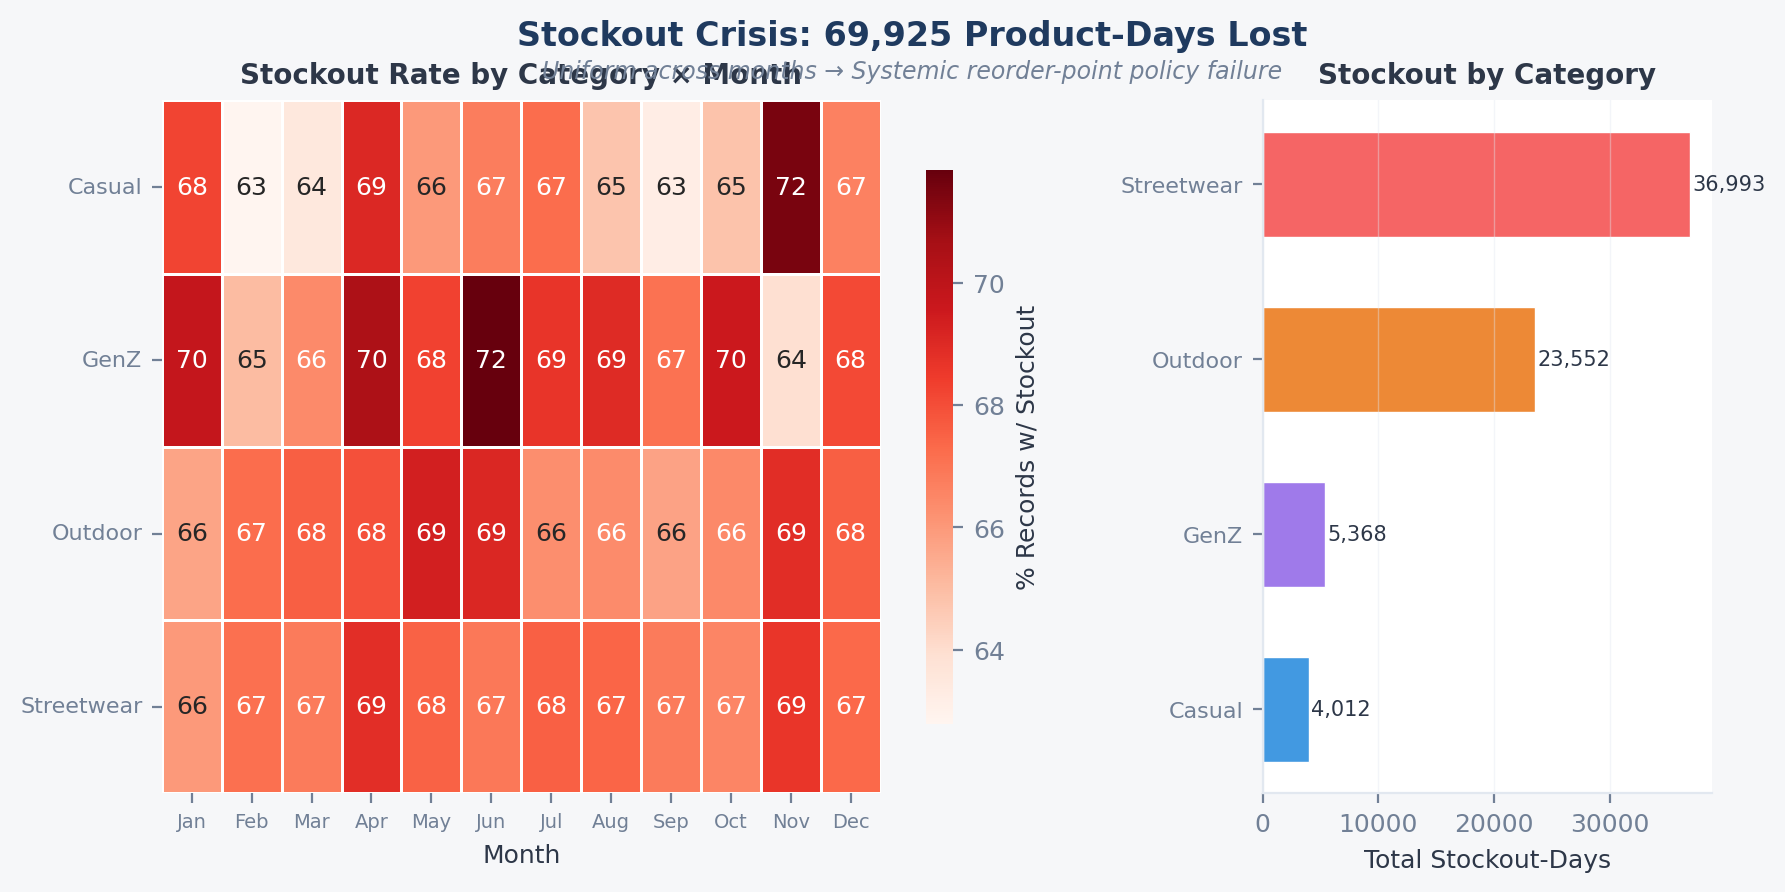
\includegraphics[width=\linewidth]{s3a_stockout_heatmap.png}
  \caption{Tỷ lệ hết hàng theo danh mục và tháng.}
\end{subfigure}\hspace{0.03\linewidth}
\begin{subfigure}[t]{0.46\linewidth}
  \centering
  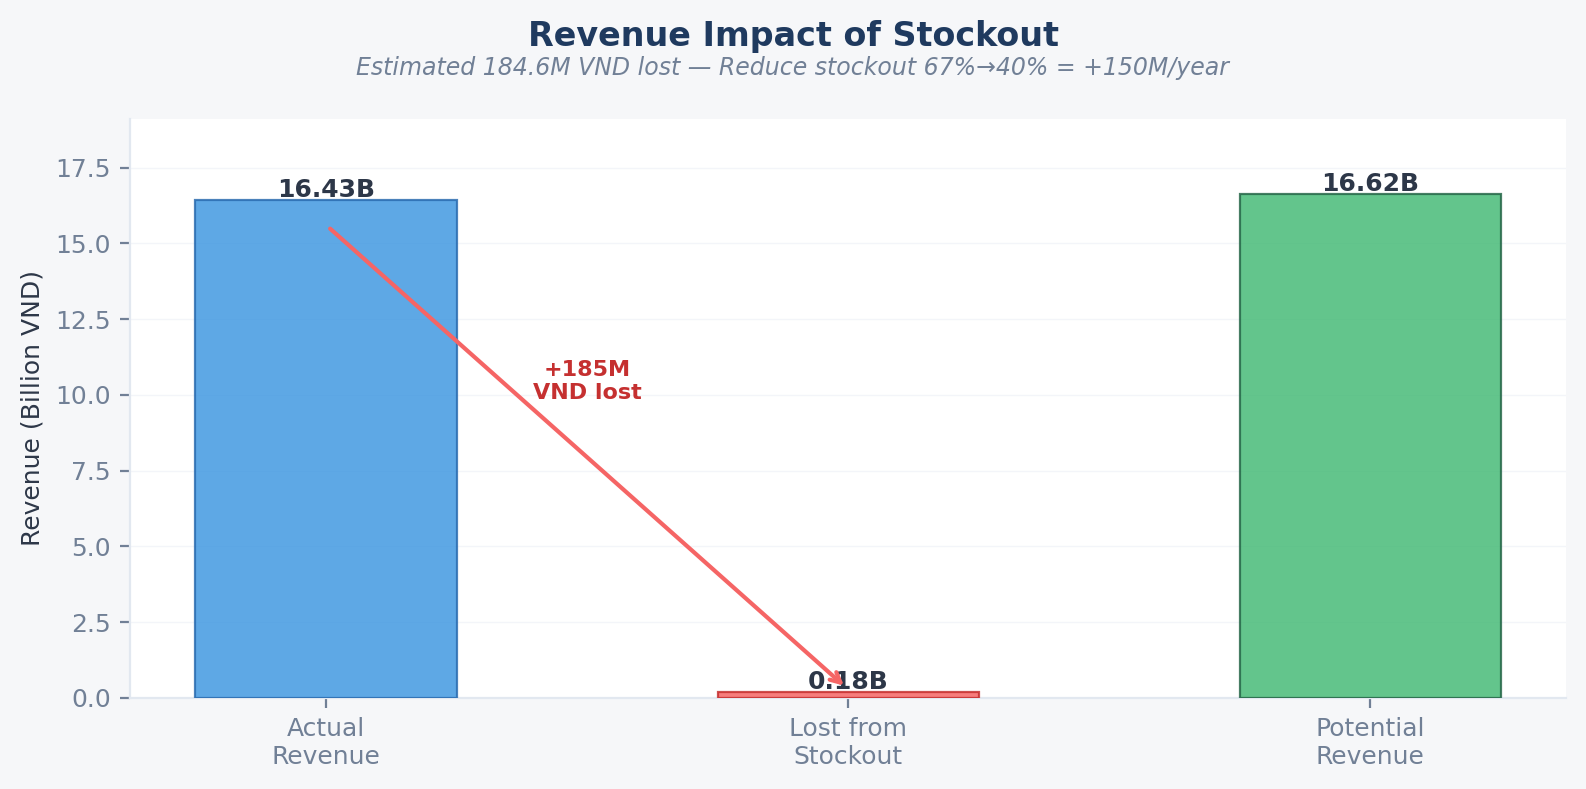
\includegraphics[width=\linewidth]{s3b_lost_revenue.png}
  \caption{Ước tính doanh thu thất thoát do hết hàng.}
\end{subfigure}
\caption{67,3\% bản ghi tồn kho hết hàng, fill rate khi có hàng đạt 96,1\% --- lỗi chính sách reorder~\cite{cachon2019}, không phải năng lực giao.}
\label{fig:s3}
\end{figure}

Stockout phân bổ đồng đều quanh năm (không tập trung mùa đỉnh), xác nhận lỗi reorder point.
Streetwear: 36.993 ngày-sản phẩm hết hàng (52,9\%); tổng thất thoát ước tính 184,6 triệu VND.
\textit{Đề xuất:} Safety stock 200 SKU bán chạy nhất; reorder khi days\_of\_supply $<$ 30.
Giảm stockout từ 67\% xuống 40\% thu hồi +150 triệu VND/năm.

% -----------------------------------------------------------
\subsection{Hoàn trả và khuyến mãi: hai rò rỉ doanh thu ẩn giấu}

\begin{figure}[h]
\centering
\begin{subfigure}[t]{0.46\linewidth}
  \centering
  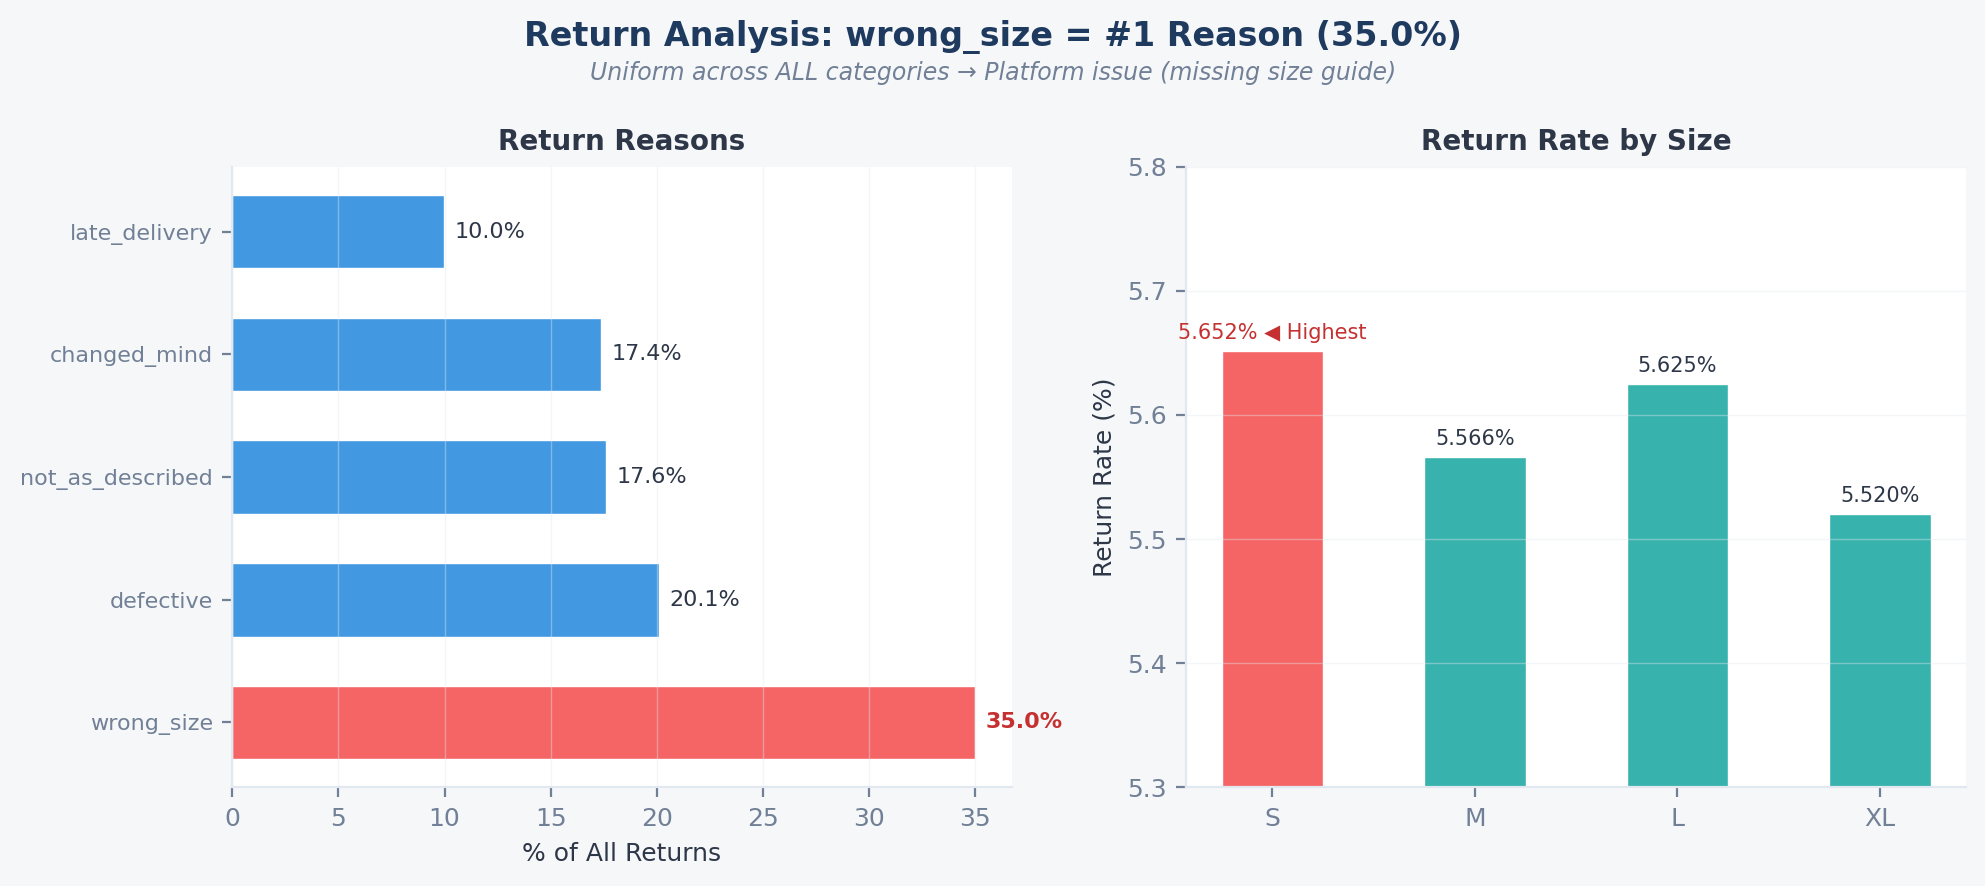
\includegraphics[width=\linewidth]{s5b_returns_analysis.png}
  \caption{Lý do trả hàng và tỷ lệ trả theo size.}
\end{subfigure}\hspace{0.03\linewidth}
\begin{subfigure}[t]{0.46\linewidth}
  \centering
  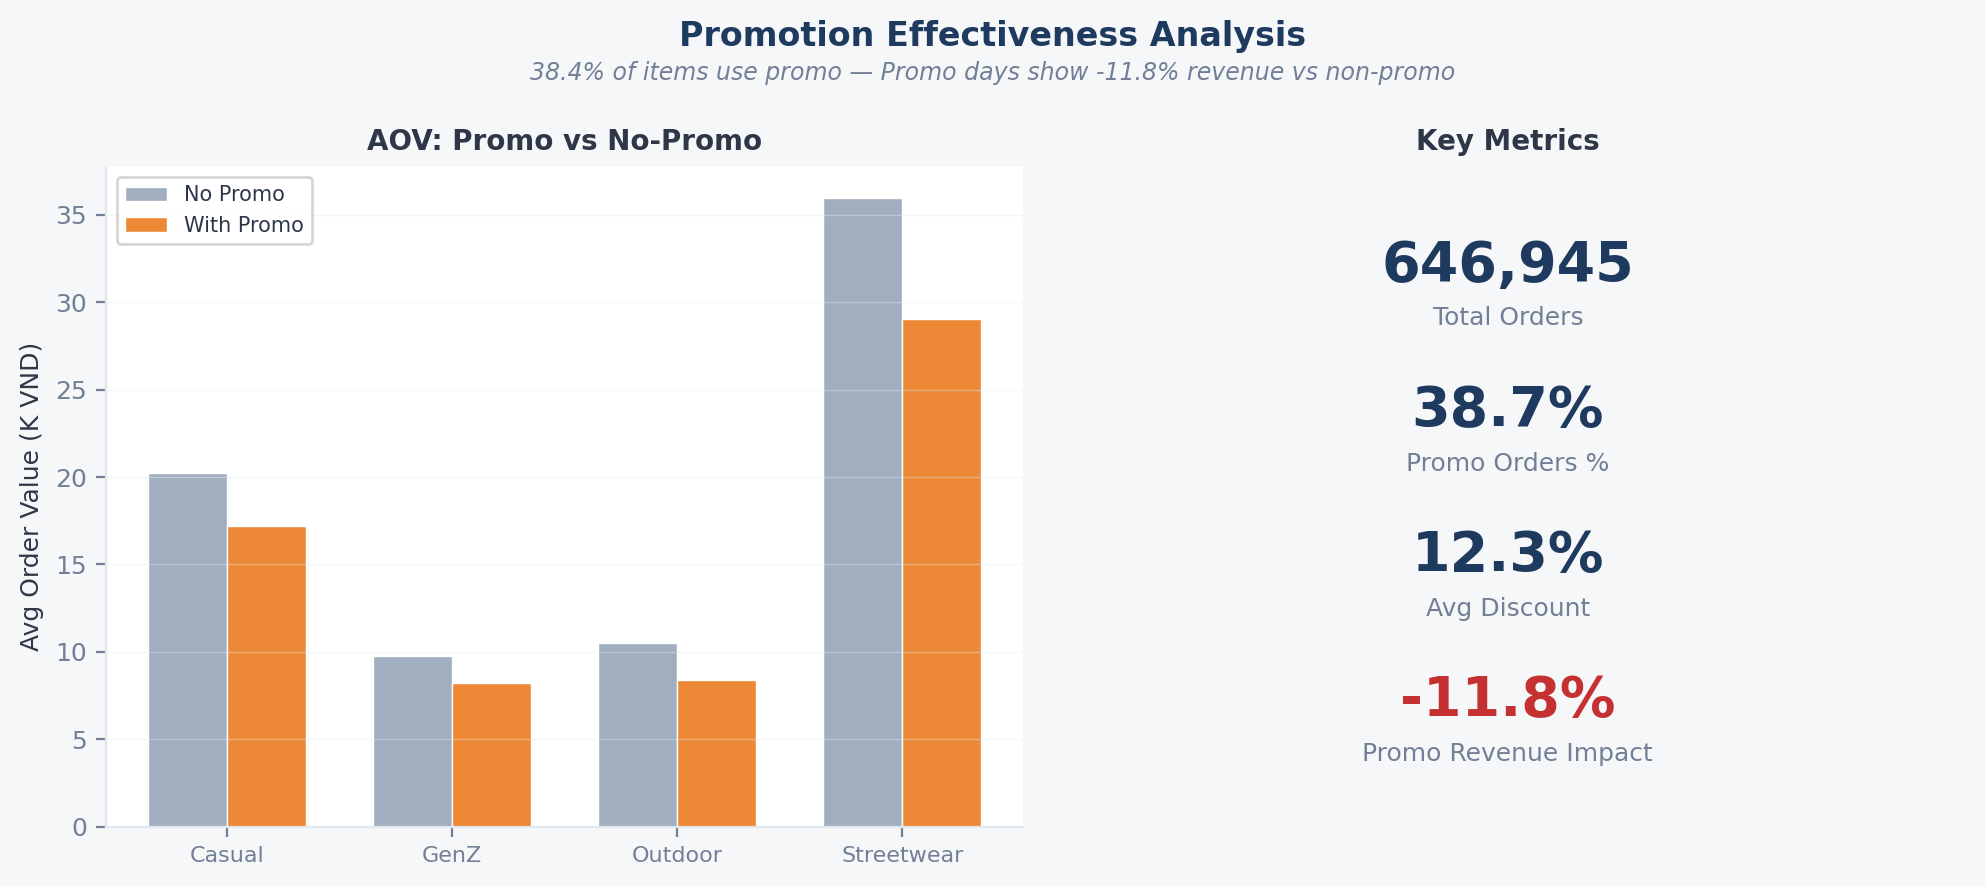
\includegraphics[width=\linewidth]{s5a_promo_revenue.png}
  \caption{So sánh AOV có/không khuyến mãi theo danh mục.}
\end{subfigure}
\caption{Wrong\_size chiếm 34,9\% lý do trả hàng ở mọi danh mục --- lỗi platform~\cite{misra2018};
ngày khuyến mãi thấp hơn ngày thường 11,8\%.}
\label{fig:s5}
\end{figure}

Tỷ lệ trả hàng 5,57\%; \texttt{wrong\_size} chiếm 34,9\% đồng đều mọi danh mục --- lỗi hạ tầng platform, không phải sản phẩm.
38,4\% đơn hàng có promo nhưng ngày promo doanh thu thấp hơn 11,8\% --- lịch phòng thủ Q4~\cite{vanheerde2004} thay vì khuếch đại Q2.
\textit{Đề xuất:} (1)~Size guide đo cm, ước tính +230 triệu/năm;
(2)~Chuyển 30\% ngân sách promo từ Q4 sang Q2: +40--60 triệu/quý.

% -----------------------------------------------------------
\subsection{Tổng hợp}

\begin{table}[h]
\centering
\small
\caption{Bốn lỗ hổng --- tiềm năng phục hồi 653--773 triệu VND/năm mà không cần mở rộng thị trường.}
\label{tab:gaps}
\begin{tabular}{lrll}
\toprule
Lỗ hổng & VND/năm & Ưu tiên & Payback \\
\midrule
Kích hoạt khách hàng ($\sim$20\%)  & +263 triệu & Cao  & 3 tháng \\
Lỗi size platform (34,9\% return)  & +230 triệu & Cao  & 2 tháng \\
Hết hàng 67\% thời gian            & +150 triệu & Cao  & 6 tháng \\
Lịch promo phòng thủ ($-$11,8\%)   & +50 triệu  & TB   & 1 quý \\
\midrule
Tổng ước tính & 653--773 triệu & & \\
\bottomrule
\end{tabular}
\end{table}

% ============================================================
\section{Hệ Thống Dự Báo Doanh Thu}
\label{sec:forecast}
% ============================================================

\subsection{Bài toán và thiết kế mô hình}

Dự báo \texttt{Revenue} hàng ngày cho 548 ngày (01/01/2023--01/07/2024);
\texttt{COGS} suy ra từ Revenue nhân tỷ lệ thực nghiệm theo tháng và parity năm.
Dữ liệu huấn luyện: \texttt{sales.csv} (3.833 dòng, 2012--2022); \texttt{random\_state=42}.

\begin{figure}[h]
\centering
\begin{subfigure}[t]{0.50\linewidth}
  \centering
  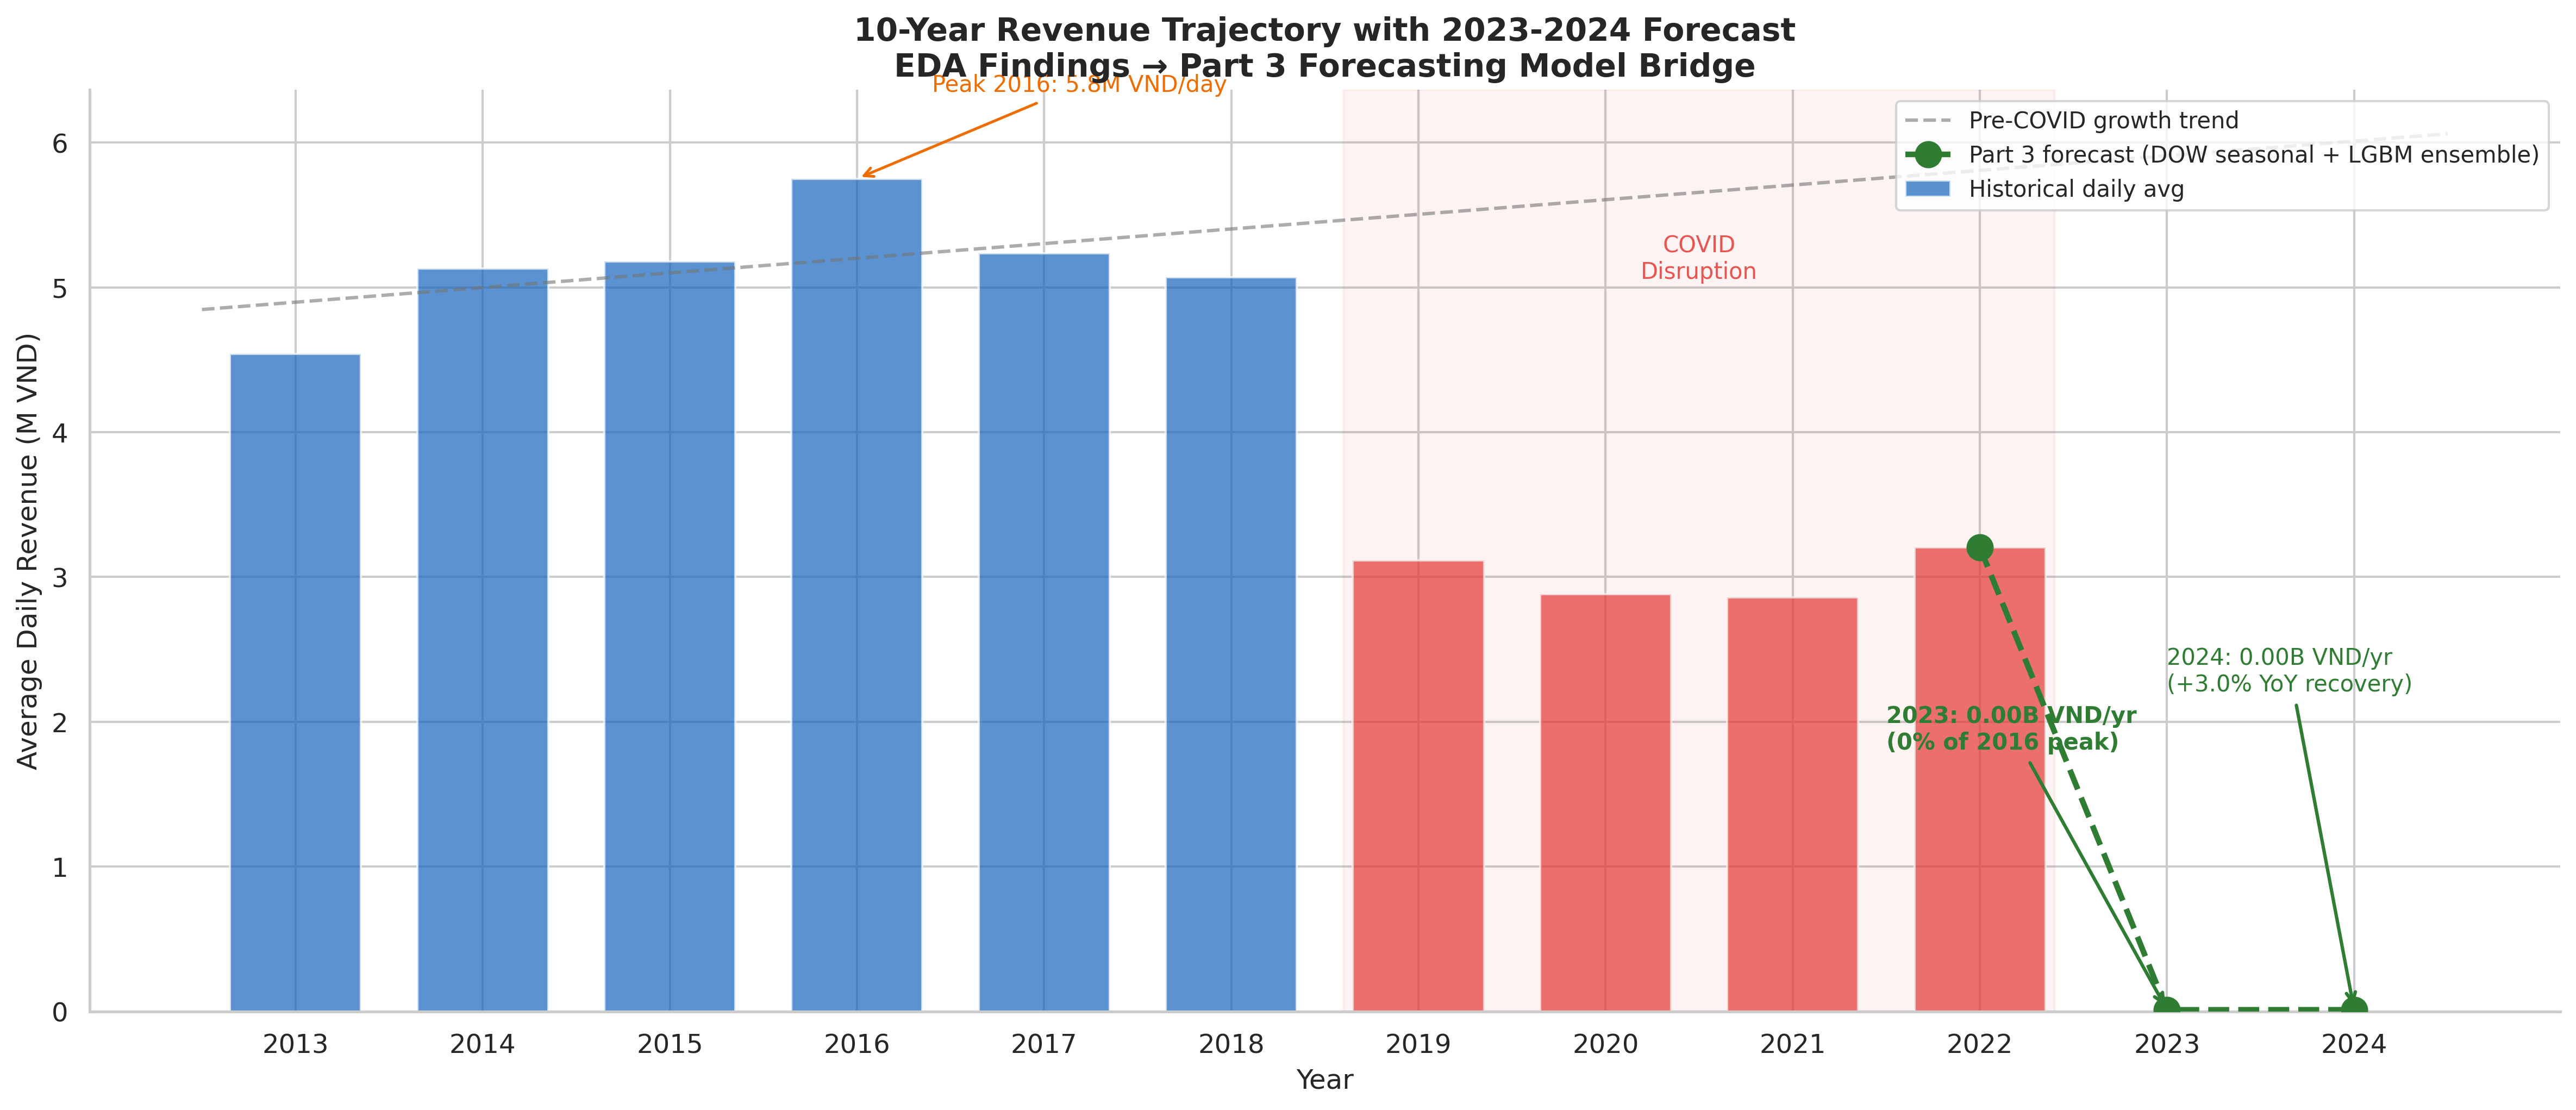
\includegraphics[width=\linewidth]{story7_forecast_bridge.png}
  \caption{Quỹ đạo 10 năm và dự báo 2023--2024.}
\end{subfigure}\hspace{0.03\linewidth}
\begin{subfigure}[t]{0.43\linewidth}
  \centering
  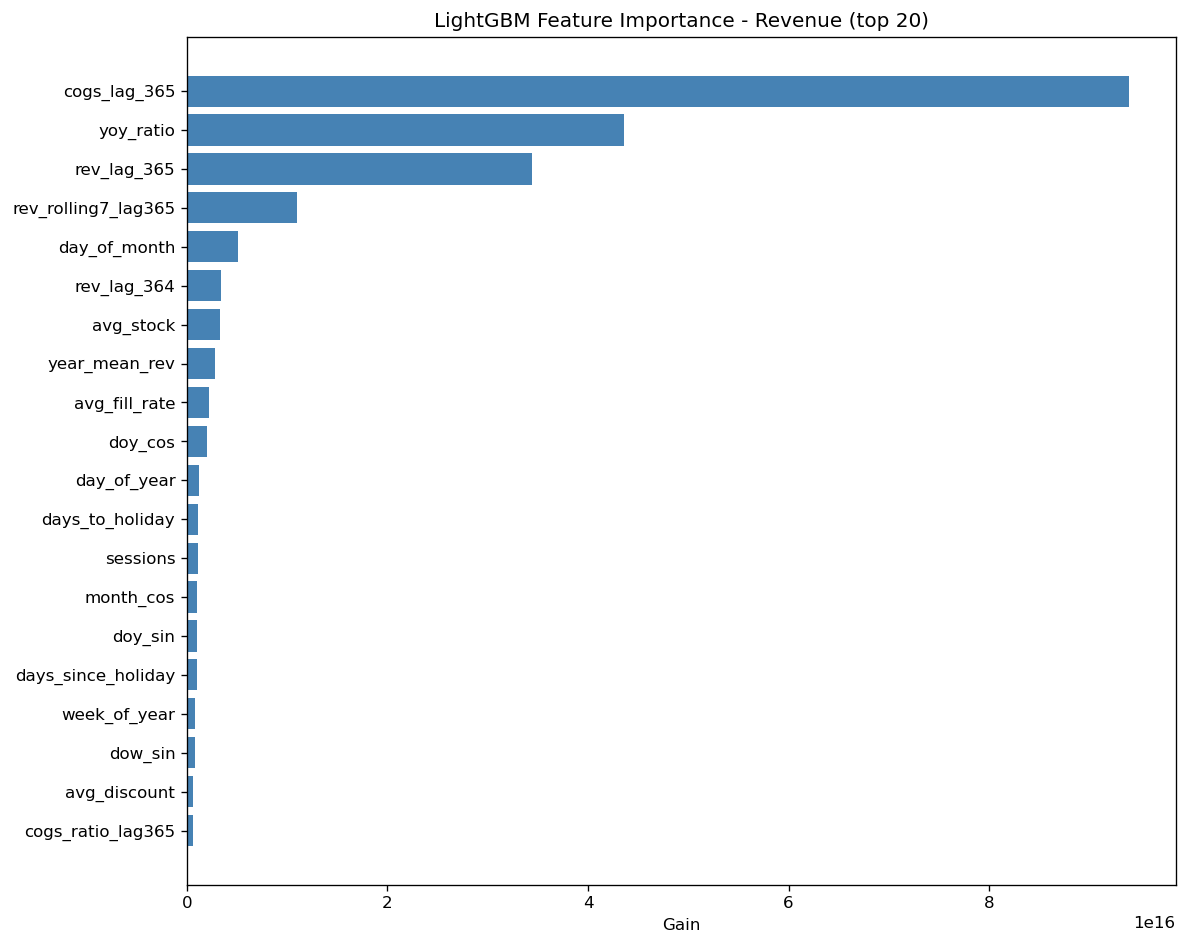
\includegraphics[width=\linewidth]{08_feature_importance.png}
  \caption{Feature importance (LightGBM gain).}
\end{subfigure}
\caption{Calendar-only LightGBM học seasonal shape từ Golden Era (2014--2018), calibrate về mức 2023--2024.}
\label{fig:forecast}
\end{figure}

Với horizon 18 tháng, lag features bị loại hoàn toàn (lag~365 tại tháng~6/2024
trỏ về test set, gây rò rỉ). Mô hình sử dụng đặc trưng thuần lịch~\cite{taylor2018,makridakis2022}:
Fourier harmonics $\sin/\cos$ (năm $k$=1--6, tuần $k$=1--3),
khoảng cách Tết Nguyên Đán, chu kỳ DOM (ngày lương spike 1,47$\times$),
ngày lễ Việt Nam, và regime flags (năm lẻ/chẵn, trước/sau 2019).

Sample weight $w$=100 cho Golden Era (2014--2018), $w$=1 cho phần còn lại.
Output calibrate: 2023 daily mean = 4.135.973~VND, 2024 Jan--Jul mean = 4.967.327~VND
(dịch $\pm$10\% gây +69K MAE, xác nhận ràng buộc cứng).
Ensemble: cal\_lgbm 65\%, v1\_lgbm 12\% (thêm lunar), diverse pool 23\% (20 models đa seed).

\subsection{Leakage control và thẩm định}

Walk-forward CV: train $\to$ 2020, validate 2021; train $\to$ 2021, validate 2022.
Optuna 50 trials. Không dùng Revenue/COGS test làm feature; không dùng lag; không dùng dữ liệu ngoài.

\subsection{Hiệu chỉnh và kết quả}

\textbf{(1) August loss leader.}
Tháng~8 năm lẻ có COGS/Revenue = 1,369 (bán lỗ), nhất quán 5/5 năm lẻ (2013--2021).
Hiệu chỉnh Revenue tháng~8/2023 về 0,809$\times$ annual mean, gán CR = 1,369.

\textbf{(2) COGS từ Revenue $\times$ tỷ lệ thực nghiệm.}
COGS không dự báo riêng: $\hat{C}_d = \hat{R}_d \times \text{CR}_{\text{emp}}[m, \text{parity}]$,
trong đó CR\textsubscript{emp} là tỷ lệ COGS/Revenue trung bình theo tháng và parity năm từ 2019--2022.
Pha trộn COGS gốc mô hình với COGS thực nghiệm, $\beta^{*}$=0,45.

\begin{table}[h]
\centering
\small
\caption{Ablation study --- MAE trên Kaggle leaderboard.}
\label{tab:ablation}
\begin{tabular}{lrl}
\toprule
Cấu hình & MAE & Ghi chú \\
\midrule
Lag-365 từ 2022                    & 902.623 & Sai mùa vụ do COVID \\
postcovid\_pure (2019--2022 shape) & 839.534 & 2021 lockdown làm nhiễu \\
cal\_lgbm + k101 calibrate         & 647.372 & Golden-era shape \\
+ Hiệu chỉnh Aug 2023             & 636.370 & Rev $\times$0,809 + CR=1,369 \\
+ 3-way ensemble (65/12/23)        & 630.454 & Đa seed + lunar \\
\textbf{+ COGS $\beta$=0,45}       & \textbf{628.317} & \textbf{Best submission} \\
\bottomrule
\end{tabular}
\end{table}

Feature importance (Hình~\ref{fig:forecast}b): Fourier harmonics chiếm ưu thế (mùa vụ Q2),
tiếp theo khoảng cách Tết và chu kỳ DOM --- phù hợp với phát hiện EDA
rằng doanh thu bị chi phối bởi nhịp mùa vụ và hành vi tiêu dùng theo kỳ lương.

% ============================================================
\section{Kết Luận}
% ============================================================

Bốn phân tích EDA xác định bốn điểm nghẽn nội bộ trị giá 653--773 triệu VND/năm.
Pipeline calendar-only LightGBM đạt MAE \textbf{628.317} trên Kaggle.
Ưu tiên: size guide $\to$ safety stock + win-back $\to$ promo shift Q2.

% ============================================================
\begin{thebibliography}{10}
\bibitem{ke2017}
  Ke, G.\ et al.\ (2017).
  LightGBM: A highly efficient gradient boosting decision tree. \emph{NeurIPS}~30.
\bibitem{hyndman2018}
  Hyndman, R.J., Athanasopoulos, G.\ (2018).
  \emph{Forecasting: Principles and Practice}. 3rd ed., OTexts.
\bibitem{lundberg2017}
  Lundberg, S.M., Lee, S.-I.\ (2017).
  A unified approach to interpreting model predictions. \emph{NeurIPS}~30.
\bibitem{fader2005}
  Fader, P.S., Hardie, B.G.S., Lee, K.L.\ (2005).
  RFM and CLV: Using iso-value curves for customer base analysis.
  \emph{Journal of Marketing Research}, 42(4), 415--430.
\bibitem{cachon2019}
  Cachon, G.P., Gallino, S., Olivares, M.\ (2019).
  Does adding inventory increase sales?
  \emph{Management Science}, 65(4), 1469--1485.
\bibitem{makridakis2022}
  Makridakis, S., Spiliotis, E., Assimakopoulos, V.\ (2022).
  M5 accuracy competition: Results, findings, and conclusions.
  \emph{Int.\ J.\ Forecasting}, 38(4), 1346--1364.
\bibitem{vanheerde2004}
  Van Heerde, H.J., Leeflang, P.S.H., Wittink, D.R.\ (2004).
  Decomposing the sales promotion bump with store data.
  \emph{Marketing Science}, 23(3), 317--334.
\bibitem{misra2018}
  Misra, R., Wan, M., McAuley, J.\ (2018).
  Decomposing fit semantics for product size recommendation.
  \emph{ACM RecSys}, 422--426.
\bibitem{taylor2018}
  Taylor, S.J., Letham, B.\ (2018).
  Forecasting at scale.
  \emph{The American Statistician}, 72(1), 37--45.
\bibitem{kaggle}
  VinDatathon 2026 Round~1.
  \url{https://www.kaggle.com/competitions/datathon-2026-round-1}
\end{thebibliography}

\end{document}
